% !TeX root = ../thuthesis-example.tex

\chapter{引言}

\section{研究背景}
张量可以被用于描述事物之间的线性关系,张量代数则是作用在张量上,对张量所表示关系进行分析的数学工具。
比如在线性系统中,使用二维张量(矩阵)表示系统状态,用矩阵变换表示系统与环境的交互。如果把张量的每个维度看做一种数据,那么张量就可以表示
这些不同种数据之间的关系。比如,在图~\ref{fig:intro}中,利用矩阵乘法即可完成作者引用文章的分析。相似的,社交网络中不同群体的关系,金融计算中不同
交易主体之间的交易信息等,都可以利用张量表示并利用张量代数进行分析。
\begin{figure}
  \centering
  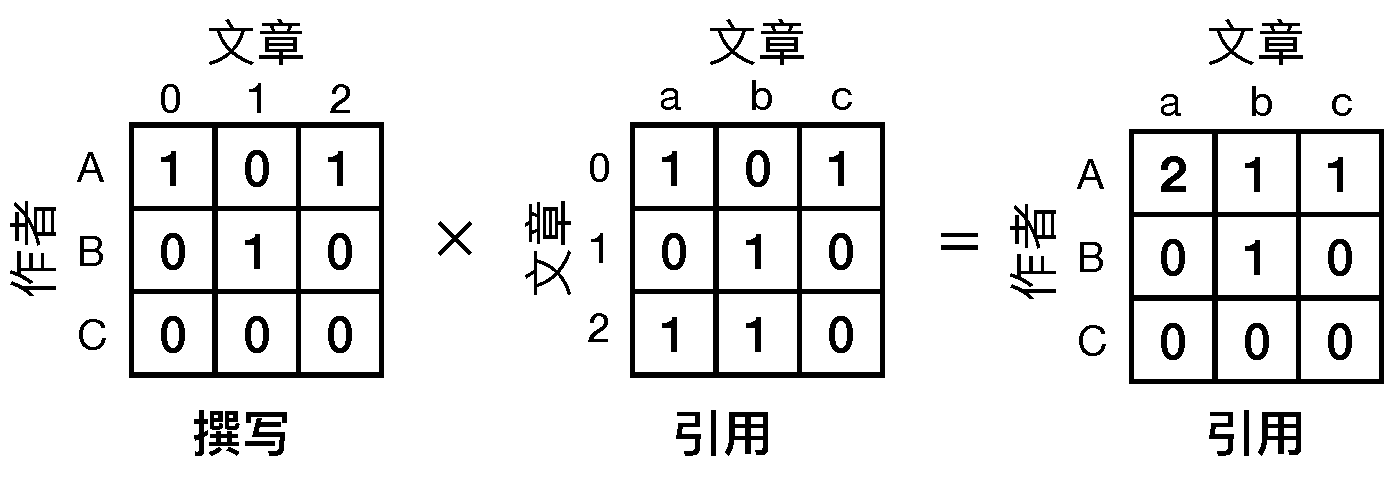
\includegraphics[width=0.99\linewidth]{intro.pdf}
  \caption{稀疏张量代数示例。第一个矩阵的第一维表示作者,第二维表示文章,矩阵表示的关系是作者写文章。第二个矩阵的第一维表示文章,第二维表示文章,矩阵表示的关系是文章引用文章。
  两个矩阵做矩阵乘法运算后得到的矩阵第一维表示作者,第二维表示文章,关系则变为作者引用文章。}
  \label{fig:intro}
\end{figure}

在现实应用中,因为稀疏关系是普遍存在的\cite{uzzi2007small},所以张量通常是稀疏的。比如在深度神经网络中,不同神经元间连接是稀疏的,体现在权重张量上就是其大部分($50\% \sim 90\%$)可以是零\cite{wang2021dual}。
再比如以及记录亚马逊网站截至2013年3月的横跨18年的用户数据的三维张量中,每一个非零元素对应近80亿个零元\cite{mcauley2013hidden}。
随着稀疏性在神经网络的广泛应用\cite{xiao2022smoothquant},以及现实生活中关系数据的日益增长,需要研究更高效的稀疏张量运算。

然而,高效稀疏张量运算面临来自稀疏格式、代数表达、优化技巧和硬件平台四方面的复杂度\cite{kjolstad:2020:phd-thesis},目前的算子库模式解决这些问题代价过大。与稠密矩阵不同,稀疏矩阵采用压缩格式存储,而算子库常
会采用自定义的压缩格式。这就限制了算子库的扩展性和不同算子库之间的迁移性。同时,因为算子库代数表达是固定的,所以会丧失算子融合带来的访存和计算收益。
不同稀疏张量运算可以采取相似的优化技巧,但是算子库模式就需要针对不同重复部署相同的优化技巧。

因此,本文针对优化技巧在不同稀疏张量运算的迁移问题提出更高效的稀疏编译算法,来提升算子性能同时降低部署复杂度。本文选取稀疏稠密混合代数运算范畴,基于稀疏稠密矩阵乘法提出了灵活规约优化技术,并基于灵活规约提出了扩展的稀疏稠密混合代数优化空间。
基于扩展优化空间,本文将灵活规约纳入稀疏迭代模型\cite{kjolstad:2017:taco},并提出灵活规约语义提升技术,该技术使得用户可以通过简单调度指令在任意稀疏稠密混合代数完成灵活规约扩展优化空间性能调优。
灵活规约通过灵活规约粒度和规约策略,将原有最佳GPU开源稀疏稠密矩阵乘法算子库性能平均提升1.6到2.7倍。灵活规约语义提升技术将原有稀疏算子编译器生成稀疏稠密矩阵乘法算子性能最高提升1.2倍,并在其他稀疏稠密混合代数上最高提升2.7倍。

\section{论文框架}
本文第2章介绍了稀疏稠密混合代数,针对GPU上稀疏稠密混合代数的优化技术,以及稀疏算子编译器的背景知识和相关工作。第3张介绍了算子优化和编译算法面临的主要挑战,以及本文的核心贡献。第4章阐释了灵活规约的内涵,构建了基于灵活规约的
扩展优化空间,并通过实验验证了灵活规约的有效性,探讨了优化空间的结构。第5章阐述了灵活规约语义提升技术的定义,介绍了算法流程和系统部署,并通过实验验证了灵活规约针对稀疏稠密混合代数优化的有效性。第6章总结了算子编译器的相关工作,
并为未来算子编译器研究提出可能的研究问题。
